\chapter{Methodology}\label{C:method} 
The core of this empirical study is the analysis of corpora of code written in each of the investigated languages. This analysis makes use of many static code analysis methods including the following:
\begin{itemize}
	\item Grep is used to perform regular expression searches on files. This can detect the more simple patterns explored in this paper.
	\item ANTLR (Another Tool For Language Recognition) is a tool which accepts a language grammar and a valid file in that language. From this it constructs a syntax tree to represent the file.
	\item JSClassFinder is a tool which detects class and method declarations in JavaScript code.
	\item Esprima accepts a JavaScript file as input and produces a JSON representation of the syntax tree of that file. This JSON file is then used as the input to JSClassFinder.
\end{itemize}
Each of these tools helps to extract valuable information from one of more of the languages analysed in this study.

\section{Selecting Languages}
The languages which have been explored thus far are limited to Java and JavaScript. These languages were covered first because they both have large open source communities and they differ on their native method of object inheritance which provides a good avenue for comparison. The other languages which will be explored in the remainder of the project are Lua and C\#. These are included to ensure that a wide enough variety of languages are analysed that it is possible to make conclusions about the usage of delegation and inheritance across languages.

\section{Assembling Corpora}
To analyse each language, we first needed to collect a corpus representative of that language's use in real world software development projects. In the case of Java, we adopted The Qualitas Corpus, which is a large collection of open source projects written in the Java language~\cite{QualitasCorpus}. Likewise, with JavaScript, we have adopted an existing corpus used by the team that developed JSClassFinder~\cite{JSClassFinder}.
\newline

For the other studied languages, Lua and C\#, quality existing corpora could not be found. For each of these languages, the top 25 open source projects were sourced from GitHub's "Trending this month" list for June, 2016. This source was chosen because it provides a group of projects for each language which are in active development as measured by GitHub, and which are easy to access. This helps to ensure that the analysis performed will be as relevant as possible to modern software development.

\section{Java Analysis}
Finding occurrences of classical inheritance in Java is as simple as looking for the extends keyword with a "grep" regular expression search. Finding examples of delegation and forwarding is more difficult and requires more information about the syntax tree of the program. To achieve this, each program of the corpus was passed through ANTLR which parses each file according to a lexer and parser generated from a Java grammar. ANTLR then constructs an abstract syntax tree which can then be traversed to search for relevant patterns.
\newline

The process for analysing a Java project follows a pipeline structure where each file is parsed and analysed in isolation. The resulting statistics of each file are then aggregated to form the overall statistics across the projects. This file isolation is important because the syntax trees produced by ANTLR consume large amounts of memory so it is not possible to hold all the Java files for a project in memory simultaneously.
\newline

\begin{center}
	\captionof{figure}{Java Analysis Pipeline}
	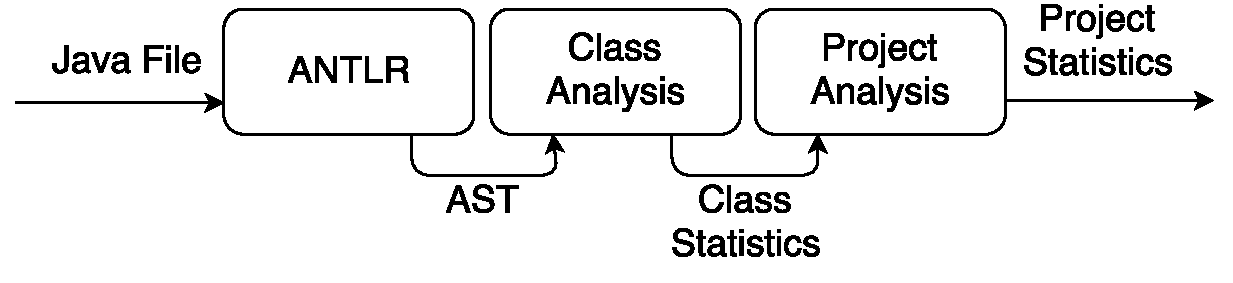
\includegraphics[scale=0.70]{AntlrPipeline.pdf}
\end{center}

\section{C\# Analysis}
As with Java, C\# was analysed using a lexer and parser generated by loading a C\# 6 grammar into ANTLR. The analysis for each project in the corpus was performed in three major passes:
\begin{enumerate}
	\item Create a syntax tree for each code file and traverse it to find all class declaration subtrees. Collect these class declarations to use in later steps.
	\item Run a visitor down each class declaration subtree, searching for all the methods and recording their modifiers. A type hierarchy is also established at this step to allow classes to find information about method calls they make which may be dispatched to a method in their superclass.
	\item Run another visitor down each class declaration tree and find constructors and check which methods are called against the modifiers found in the previous pass to determine which methods could miss their intended target under a different object initialisation model.
\end{enumerate}
The statistics gathered for each file in each project were then aggregated across the corpus to collect information about the corpus as a whole.

\section{JavaScript Analysis}
The JavaScript analysis in this study consisted mainly of a recreation of the JSClassFinder study. JSClassFinder is a tool created by a team of researchers to analyse the extent to which JavaScript developers use classes in their projects. In addition to this, Grep was used to identify use of delegation.

\section{Lua Analysis}
The Lua corpus was analysed with Grep to identify code patterns and keywords associated with class usage.






